\section{Where latency goes under load}
\label{sec:load}

\paragraph{Decode dominates each request, even with long prompts.}
We first compared a prefill-heavy workload (2048 input and 32 output tokens) with a
decode-heavy one (64 and 512), at C1 and C8. We had predicted that the prefill-heavy
workload would be dominated by the time before the first token. It was not. A request
running alone spent about 40\ms{} in prefill and about 122\ms{} in its 31 generation
steps. A simple cost estimate predicts this \citep{pope2023scaling}. Prefill of 2048
tokens needs about 1.6 TFLOP (two FLOPs per weight per token, plus attention), which
takes 21\ms{} at the A4000's dense 16-bit tensor peak of 77 TFLOPS. Each generation step
must read about 1\,GB of weights, which takes at least 2.2\ms{} at 448\,GB/s, or
68\ms{} for 31 steps \citep{nvidiaa4000}. At those ideal rates prefill would be about
a quarter of the request, so on this GPU the workload we called prefill-heavy is
decode-dominated, and the prediction could have been made from the estimate.

At C8 the share of latency before the first token rose from 31\% to 45\%, but it
stayed below half. (At C1 the client's TTFT of 54\ms{} includes about 14\ms{} of request
handling outside the server's prefill time.) Concurrency did amplify different
components in the two regimes. The decode-heavy workload gained 6.46$\times$
throughput from C1 to C8 for 10\% slower per-token time. The prefill-heavy one gained
only 2.8$\times$, with queueing and a tenfold rise in ITL p99.
% src: reports/milestone3-20261003T180358Z-phase-b.md (Result; predicted signatures table; C1 TTFT 54.4 ms, server 0.01 / 40.3 / 122.5 ms); FLOP and byte estimate from the model config (24 layers, hidden 896, MLP 4864, 0.36B non-embedding and 0.49B total parameters, bf16) and the A4000 datasheet (448 GB/s; 153.4 TFLOPS tensor with sparsity, so 76.7 dense)

A plausible reading at the time is that at C8 much of a request's decode time is spent
in engine steps that also carry other requests' prompt chunks. Under chunked prefill,
vLLM schedules running decodes and new prompt chunks in the same step, up to its token
budget. A step that carries a large chunk takes about as long as a prefill, so every
request decoding in that step sees a long inter-token gap. A per-request phase
breakdown therefore books much of the GPU's prefill work as decode time. Milestone 5's
step log fits this reading: at this prompt length, 23\% of C8 steps carried prompt
work.
% src: reports/milestone3-*-phase-b.md (Interpretation: what server decode time measures at C8); reports/milestone5p2-*-part2.md (C8 step-log table, len2048-budget2048-c8: 23%)

\paragraph{Past saturation, the added latency moves into each step.}
We then raised concurrency on the prefill-heavy workload to C16 and C32, predicting
that the time before the first token would come to dominate. The opposite happened.
The share of latency before the first token fell from 0.44 at C8 to 0.35 at C16 and
0.24 at C32. Output throughput peaked at C16 (583 tokens/s) and fell slightly at C32
(555). Median ITL went from 4.9\ms{} at C8 and 5.5\ms{} at C16 to 55\ms{} at C32
(Figure~\ref{fig:crossover}). A pre-registered sweep (C8, C12, C16, C24, C32) located
the jump between C16 (5.5\ms) and C24 (45.8\ms). It reproduced the earlier session
within about 1\% on a different machine. The jump in the median is abrupt because the
gaps form two clusters, short ones from decode-only steps and long ones from steps that
carry a prompt chunk, and the median moves from one cluster to the other once most
gaps come from prompt-carrying steps. Server decode time per output token rose more
smoothly, from 8.7\ms{} at C8 to 18.1\ms{} at C16 and 44.7\ms{} at C32.
% src: reports/milestone3-20261003T201214Z-phase-c.md (Result; crossover table; server decode 270.9 / 559.7 / 1384.8 ms over 31 steps); reports/milestone3-20261006T022744Z-phase-d.md (sweep; prediction 1; reproduction)

\begin{figure}[t]
  \centering
  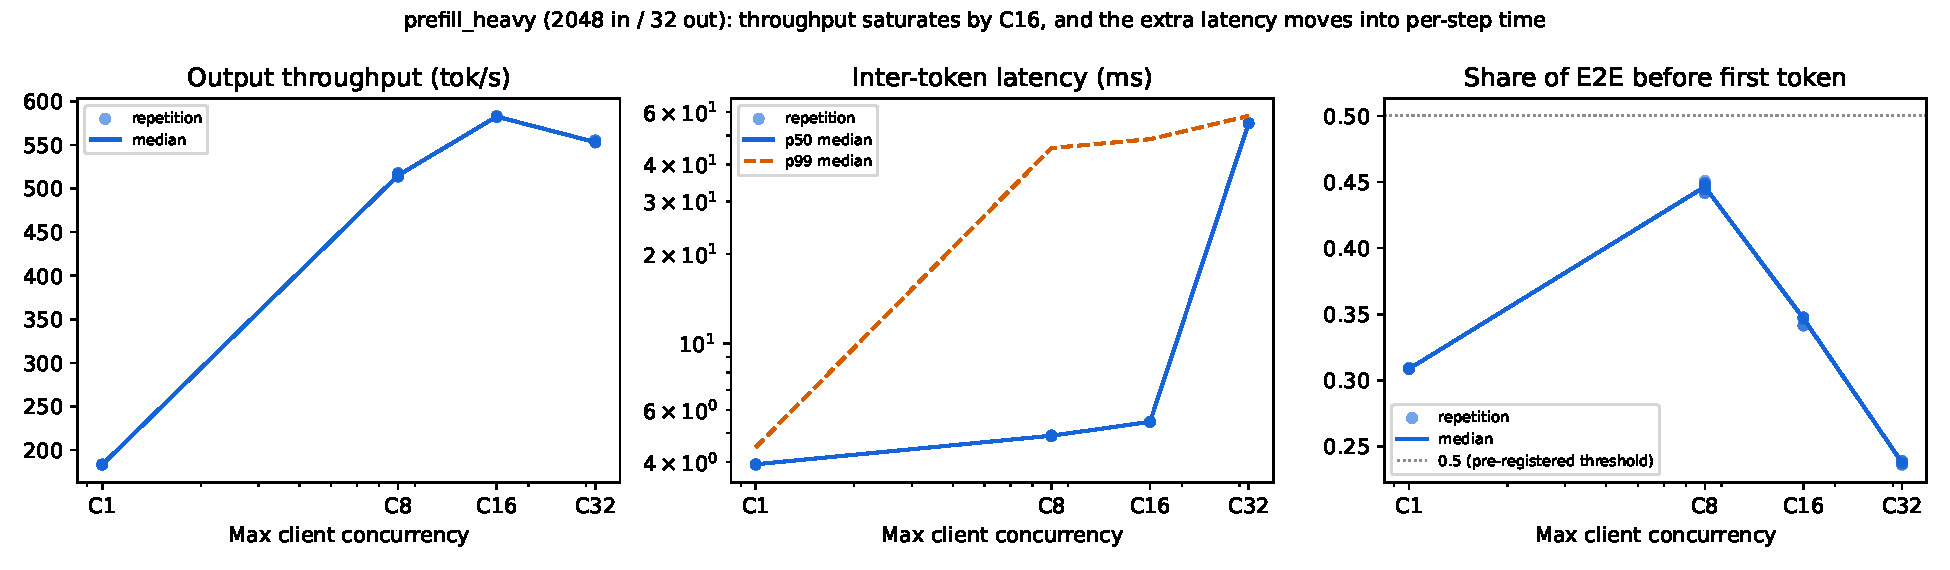
\includegraphics[width=0.78\linewidth]{milestone3-phase-c-crossover.pdf}
  \caption{Prefill-heavy workload (2048/32 tokens) against concurrency: output
    throughput, ITL p50 and p99, and the share of latency before the first token.
    Past C16, added latency appears as per-step time while the share before the
    first token falls. The C1 points and six of the twelve C8 points come from the
    contention study's control series.}
  \label{fig:crossover}
\end{figure}

\paragraph{The shift is bounded.}
At $B{=}2048$ a step carries at most one 2048-token chunk, so it costs at most about
56\ms{} (ITL p99 was 58\ms{} at C32), and a request's 31 generation steps take at most
about 1.8\,s. Past saturation throughput no longer grows, so by Little's law each added
request in flight adds latency, and once steps are full that latency must go into the
wait for the first token. Mean TTFT already doubled from C8 (215\ms) to C32
(431\ms). The per-step shift we measured therefore describes C16 to C32 at this budget,
while steps fill toward the cap. Beyond C32, and under open-loop load, we expect delay
to return to TTFT; we did not test this.
% src: reports/milestone3-20261003T201214Z-phase-c.md (crossover table: mean TTFT 215.2 / 430.9 ms; ITL p99 58.2 ms at C32); bound derived from the budget cap
